\documentclass{article}
\usepackage{amsmath}
\usepackage{graphicx}
\begin{document}

\title{Birds: Game Design}
\author{Karl Hiner, Dustin Schmidt}
\maketitle
\tableofcontents

\section{Game Overview}
\subsection{Main Objective}
Birds (yet to be named) will be a strategy game where the player is in control of a single bird amongst a flock of AI-controlled birds.  The player's primary objective is to acquire birds into their ``flock''.
\subsection{Gameplay Details}
\subsubsection{Grow Your Flock}
Birds are considered to be in the player's flock if they are within a certain radius of the player in any direction.  Birds are acquired into the player's flock by eating food and gaining ``rep''. (Maybe ``strength'' would make more sense, but I like the idea of Mob-Birds gaining rep.  They could even have fedora hats later - who knows, every game needs a Schtick!).  As the player eats more food, friendly birds become attracted to the player, and are more likely to ``flock'' with the player (fly close to the player).
\\\\
Initially, the game will be an open-ended, point-accumulating game.  Each bird in the player's flock is worth one point, and the goal is to simply set a high-score for most birds in the flock at any time.  Different modes of gameplay, such as time-trials, story-modes, etc., will be considered after the initial development stages.

\subsubsection{Beware of Hawks}
Hawks will occasionally show up to try and eat friendly birds (including the player).  The player initially has 3 health points, and will lose one health point for each strike from a hawk.  Other friendly birds, however, can only suffer one strike from a hawk, and will be removed from play after a hawk strike.

\subsubsection{Food, Nests}
Food is randomly distributed throughout the map at the beginning of the game, and will randomly spawn throughout the lifetime of the game.  Different food types will have different rep/strength values, and special types of food can also replenish one health point. (A possible gameplay component could be the need to distribute food to other birds in your flock.  Each bird could gradualy lose energy (indicated by color).  One main objective of the game could be finding food and delivering it to nests, to gain rep/whatever.  There could be a choice element of whether to spend food on gaining rep or replenishing your flock).

\section{AI Strategies}
\subsection{Collaborative Diffusion (CD)}
\subsubsection{CD Overview}
The backbone of the AI for Birds is a goal-driven technique called Collaborative Diffusion (CD).  CD can be thought of as a diffusion of scents throughout a grid.  These ``scents'' are just floating-point values that are assigned to a cell in the play-grid.  They originate at point of interest (such as a food item, or an enemy), and they spread (diffuse) throughout the map using very simple local rules.  Here are the basic steps of CD:
\\\\
For each frame (or turn):
\\
1. Assign the highest possible diffusion value to the cells that hold features of interest.  Cells can have more than one ``type'' of value, indicating different goals.
\\
2. Iterate through each cell in the play-grid.  For each cell, assign it diffusion value(s) as a weighted sum of its neighbor's diffusion values. (Optionally, some cells can be always given a diffusion value of $0$, such as walls and barriers).
\\
3. Repeat step 2 for a desired number of iterations.  The accuracy and usefullness of the diffusion grid increases with the number of iterations, so the number of iterations is usually chosen only for performance considerations.
\\
4. After determining all diffusion values for all grid cells, simply move the agents in the game (in this case, birds), to the adjascent square with the highest diffusion value corresponding to their current goal (or a weighted combination of several goals).  With enough iterations, this path approaches an optimal shortest-path from any agent to a point of interest.
\subsubsection{Benefits of Collaborative Diffusion Approach}
Not only is collaborative diffusion an efficient way to find shortest paths for many agents to many goals, but it is also known to result in unpredictable, emergent behavior, especially as many goals are being diffused.
\\\\
Division of labor can be acheived by making certain agents attracted to certain ``scents'' (diffusion goals).  For example, some agents could be dedicated explorers, while others could be dedicated to seeking out and engaging combatants.
\\\\
Dynamic goal-changing comes for free with collaborative diffusion when movement choices are made as a function of multiple diffusion value types.  Depending on game-state and circumstance, more weight can be given to different values.  For instance, food diffusion goals can be given more weight as strength decreases for a bird.  Thus, if such a weak bird is presented with a choice of following a path to food or a path to fight an enemy, food will be preferred by simply changing one weight paramater.

\subsubsection{Emergent Flock Cohesion}
Flocking behavior requires some form of cohesion to keep the flock in tact.  Collaborative Diffusion will facilitate flock cohesion through the use of two goal metrics.\\
 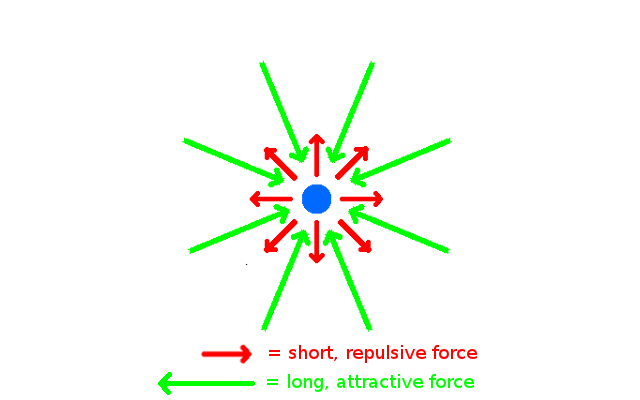
\includegraphics[width=60mm]{Bird_Forces.png}\\
Firstly birds will be attracted to other birds through a highly diffused goal.  A well fed bird will present an attractive goal to other birds.  A particular bird's attractiveness to other birds may be proportional to how well fed the attracting bird is.  Secondly each bird will have a weakly diffused anti-goal which will repel neighboring birds to maintain some degree of separation.  The repulsion anit-goal may be conceptualized as the sound of other birds squawking to maintain reasonable separation of the flock members.\\

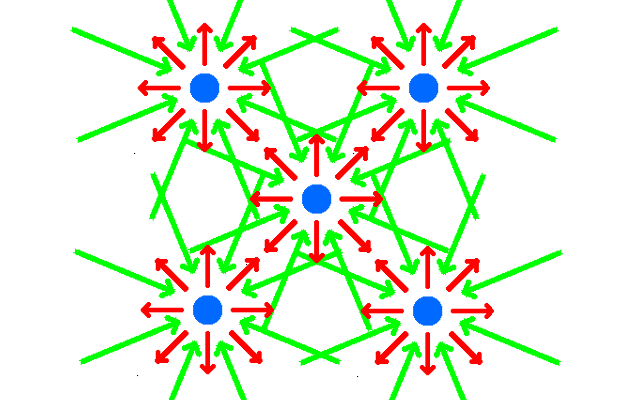
\includegraphics[width=50mm]{Bird_Forces_Multiple.png}

\section{Platform/Environment}
Birds will be written in Python, using Numpy, and possibly Scipy, for efficiency in numeric computations.
\\\\
Initially, the game will be in 2D, using the Python-included tkinter 2D library.  We plan to move to a 3D environment after this proof-of-concept phase.\\\\
Depending on Windows compatability, the following Python 3D libraries are currently being considered:\\
\subsection{Soya}: Intuitive and powerful high-level 3D library for Python.  The downside here is the lack of \textit{stable} support for Windows.\\
\subsection{PyOpenGL}: We would prefer to avoid this engine, as it is merely a wrapper around OpenGL, and has little to no high-level 3D development support. (OpenGL is a pain, and it's easy to do the wrong/inefficient thing!)\\
\subsection{PyGame}: This framework only provides 2D graphics and wrappers for OpenGL but it does afford other useful mechanisms such as efficiently updating sprites and joystick interaction.
\subsection{Panda3D}: A more modern high level 3D graphics library for Python and C++.  Provides the same features as Soya and more.  More recently maintained project than Soya\\

\section{Game Modules/Representation}
The game representation will be divided into the following components

\subsection{Frame}
	\begin{itemize}
		\item Maintains a representation of the game state (map and agents)
		\item Provides some display of the game state (2D or 3D depiction of the game)
		\item Facilitates user interaction with game state

	\end{itemize}

\subsection{Agent}
	\begin{itemize}
		\item Represents a singular entity within the gamespace
		\item Maintains information about its position
		\item Maintains a reference to the map/environment
		\item Has an update function which:
			\begin{itemize}	
				\item Reads environmental metrics about its surrounding neighborhood using its reference to the map/environment
				\item Interprets the environmental metrics to generate a new state for itself
				\item Returns some representation of an effect on its surrounding neighborhood
			\end{itemize}
	\end{itemize}

\subsection{AgentGroup}
	\begin{itemize}
		\item Represents a collection of Agents
		\item Has an update function which calls the update function of all member agents
	\end{itemize}

\subsection{Map/Environment}
	\begin{itemize}
		\item Consists of various diffused metrics associated with discrete partitions of the game space.
		\item Maintains a collection of 2D/3D numpy arrays, one array per environmental metric
		\item Maintains a diffusion rate applicable to each array/metric
		\item Provides a method for diffusing each metric array
		\item Provides a method for retrieving the environmental metrics for some neighborhood of a point in the gamespace
		\item Provides a method of mapping from continuous gamespace into discrete spatial partitions
	\end{itemize}


\section{Project Plan}
\subsection{Phase 1 - 2D Prototype - 9/24/12 to 10/12/12}
Construct a prototype to develop understanding about the problem space.
\begin{itemize}
	\item Use a numpy array to store goal information
	\item Implement some method of diffusing the goal information through out the array
	\item Construct agents which act upon goal information
	\item Provide a 2D graphical depiction of the game state
	\item Explore representation options
\end{itemize}

\subsection{Phase 2 - Refinement - 10/15/12 to 11/9/12}
\begin{itemize}
	\item Decompose prototype into distinct game modules
	\item Provide continuous representation of game entities while maintaining discretized representations of goals
	\item Introduce PyGame elements
		\begin{itemize}
		\item Employ PyGame Sprite and Group modules to implement Agent and AgentGroup
		\item Introduce Joystick as optional UI input
		\end{itemize}
	\item Begin experiments with multiple agents with differing strategies/objectives
	\item Begin experiements with goal layers:
		\begin{itemize}
			\item Map can store and diffuse multiple layers
			\item Agents can employ strategies which act on multiple layers
			\item Environment can selectively display multiple layers
		\end{itemize}
	\item Begin explorations in 3D environments
\end{itemize}

\subsection{Phase 3 - Extend to 3D - 11/9/12 to }
\begin{itemize}
	\item Make it pretty... (more detail to come)
\end{itemize}




\end{document}